\documentclass[]{ANStopical}
% M&C 2027 full paper - ANS topical template (ANStopical.cls).
% Rules: max 10 pages including references, figures and tables; abstract 200-250
% words; up to 5 keywords; no headers, footers, page numbers or hyperlinks in the
% final PDF; PDF size <= 4 MB; figure text >= 10 pt.
% Every number in this paper comes from the notebook FM_burnup_criticality_search.ipynb.

\usepackage{booktabs}
\usepackage{siunitx}

\title{A Burnup Correction Ratio for the Fission Matrix Criticality Search in Heat-Pipe Micro Reactors}

%%% TODO: confirm the author list and the affiliations before submission
\addAuthor[christian.vita@polito.it]{Christian Vita}{1}
\addAuthor{Nicol\`o Abrate}{1}
\addAuthor{Sandra Dulla}{1}
\addAuthor{Valerio Mascolino}{2}
\addAuthor{William Walters}{3}
\addAuthor{Nicolas E. Stauff}{2}
\addAuthor{Fausto Franceschini}{3}

\addAffiliation{1}{Politecnico di Torino, Dipartimento Energia, Torino, Italy}
\addAffiliation{2}{Argonne National Laboratory, Lemont, IL, USA}
\addAffiliation{3}{Westinghouse Electric Company, Cranberry Township, PA, USA}

\Abstract{%
The fission matrix (FM) method turns the criticality search of a heat-pipe micro reactor (HPMR) into the eigenproblem of a small matrix, interpolated from a database of Monte Carlo tallies. In previous work the database was built over the fuel temperature and the control-drum angle, and the critical drum position at any power is found in a fraction of a second. This paper adds fuel burnup to the method without adding a third axis to the database. The burnup effect is factorized out of the interpolated matrix through a multiplicative Burnup Correction Ratio (BCR): the element-wise ratio between the matrix tallied at a burnup snapshot and the matrix tallied at the fresh state, both at fixed reference conditions. One low-statistics depletion of the VTB HPMR model at nominal power gives the compositions; twelve independent full-statistics transport calculations, restarted from it, tally the snapshot matrices at about 66 CPU\,h each. The statistical uncertainty of both databases is propagated to every result with an ensemble of fifty database realizations, in which each coefficient is perturbed independently within its tally uncertainty. Over a 66-month cycle at \SI{2}{MW} the critical drum angle moves from \ang{62} to \ang{12}. Reference Serpent 2 calculations at the states returned by the algorithm give $k_{\rm eff}$ within $-59$ to $-5$ pcm of unity, with the same bias as at beginning of life. The three assumptions of the factorization -- angle-independent, frozen-temperature and single-history BCR -- are measured with dedicated campaigns and found at or below that residual. A full cycle costs 18 seconds on one core.
}

\keywords{fission matrix, criticality search, burnup, heat-pipe micro reactor, Monte Carlo}

\shortTitle{A Burnup Correction Ratio for the Fission Matrix Criticality Search}
\authorHead{C. Vita, et al.}

\begin{document}

\section{Introduction}\label{sec:intro}

Heat-pipe micro reactors (HPMRs) are controlled by rotating drums in the radial reflector. Their design and operation need many criticality searches: at every power level and at every stage of the fuel cycle, the drum angle that makes the core critical must be found together with the temperature field it produces. A full-core Monte Carlo calculation per search is affordable for a few states, not for the thousands that a design space or a cycle analysis require.

The fission matrix (FM) method \cite{carney2014,walters2018rapid} offers a way out. The core is divided into $N$ cells. A single criticality calculation tallies the matrix $A$, whose element $a_{ij}$ is the number of fission neutrons produced in cell $i$ per fission neutron born in cell $j$. The fundamental eigenpair of $A$ gives $k_{\rm eff}$ and the cell-wise fission source $F$,
\begin{equation}
    k_{\rm eff}\,F = A\,F ,
    \label{eq:fm}
\end{equation}
at the cost of an $N\times N$ eigenproblem. The matrix depends on the state of the core: temperatures, absorber positions, compositions. The method becomes predictive when a database of tallied matrices covers the states of interest and the matrix at any other state is interpolated from it.

In previous work \cite{vita2025fim4ntra,vita2026fm} such a database was built for the VTB HPMR model \cite{ortensi2024hpmr} over two axes, the fuel temperature and the control-drum angle, and a criticality search algorithm was built around it. A power-to-temperature correlation stands in for the thermal solver. The critical drum angle at any power is obtained in a fraction of a second, with $k_{\rm eff}$ within a few tens of pcm of reference Serpent 2 calculations \cite{leppanen2015serpent}. Burnup was left out. Fuel depletion changes the FM coefficients through the composition, and a cycle analysis needs those changes: the drum angle that keeps the core critical, the remaining excess reactivity and the cycle length. Burnup-dependent FM methods exist, for example the burnup algorithm of the RAPID code system \cite{pungercic2023brapid} and the combined FM depletion coupling of Ref.~\cite{he2024combined}. The question here is different: how to add burnup to a database that already spans temperature and drum angle, without multiplying its size.

This paper proposes a factorization. The interpolated matrix is multiplied element-wise by a Burnup Correction Ratio (BCR): the ratio between the matrix tallied at a burnup snapshot and the matrix tallied at the fresh state, under fixed reference conditions. The BCR is tallied once per snapshot time, at a single drum angle and at the nominal temperature state, and applied at every state the search visits. Section~\ref{sec:fm} recalls the FM criticality search. Section~\ref{sec:bcr} states the database-size problem, defines the BCR and describes the snapshot campaign and its cost. Section~\ref{sec:uq} describes how the statistical uncertainty of the databases is propagated to the results. Section~\ref{sec:results} presents the cycle, its verification against reference calculations and the measurement of the three assumptions behind the factorization. The study is done at the nominal power of \SI{2}{MW}. Nothing in the construction depends on the power: the temperature axis of the database carries the power dependence, so the extension to other power levels is immediate.

\section{The Fission Matrix Criticality Search}\label{sec:fm}

\subsection{Generation of the fission matrix}

The VTB HPMR model has 30 fuel assemblies and 12 control drums in the radial reflector, a heavy-metal inventory of \SI{448.5}{kg} and a nominal power of \SI{2}{MW}. Each assembly is split into three axial zones, so $N = 90$. The FM is tallied by Serpent 2 during a criticality calculation: each cell is a material zone of the input, and the code accumulates, for every source cell $j$, the fission neutrons produced in every cell $i$. The output is the $90\times 90$ matrix $A$ and the relative statistical uncertainty of each coefficient.

The database of Ref.~\cite{vita2026fm} (FMDB) has 8 fuel temperature levels and 17 drum angles, from \ang{0} (absorber fully extracted) to \ang{180} (absorber facing the core): 136 criticality calculations. Each one runs $10^5$ neutrons per cycle, 500 active and 30 inactive cycles, and costs about 63 CPU\,h; the median relative uncertainty of the coefficients is \SI{9}{\percent}. The matrix at any state is obtained by bivariate linear interpolation, $\tilde a_{ij}(T_{f,i},\theta)$: the fuel temperature of the target cell $i$ selects the position on the temperature axis, the drum angle $\theta$ the position on the angle axis.

\subsection{The search}

The search of Ref.~\cite{vita2026fm} is not changed by the burnup extension. Two nested loops surround the interpolated matrix. The inner loop finds the neutronic--thermal equilibrium at fixed drum angle. The fuel temperature of every cell is obtained from the current fission source through a linear power-to-temperature correlation; at nominal power its parameters map the source distribution onto the \SIrange{823}{874}{K} range of the reference multiphysics solution. The matrix is interpolated at the new temperatures, Eq.~\eqref{eq:fm} is solved, and the loop repeats until the temperature profile changes by less than \SI{0.5}{\percent}. The outer loop is a bisection on the drum angle in $[\ang{0},\ang{180}]$. For scans, the stopping criterion is deterministic, $|k_{\rm eff}-1| < 1$ pcm. When the uncertainty ensemble of Section~\ref{sec:uq} is active, the search stops when the $\pm 1\sigma$ band of the last two iterates contains $k_{\rm eff}=1$: the drum angle is not resolved beyond the statistical resolution of the database. If the core is subcritical with the drums fully extracted, criticality cannot be restored. This guard, added for the present work, defines the end of cycle life.

At beginning of life (BOL) and nominal power the search converges in 12 outer iterations and \SI{0.5}{s} on one core, ensemble included. The result is $\theta_{\rm crit} = 62.31 \pm \ang{0.14}$ with $k_{\rm eff} = 1.00004 \pm 11$ pcm. A reference Serpent 2 calculation at that state gives $k_{\rm eff} = 1.00060 \pm 12$ pcm. The deviation, $-56 \pm 16$ pcm, is the $(T,\theta)$ interpolation residual of the database; it is met again along the cycle. The Reflector Correction Ratio of Ref.~\cite{vita2026fm}, which corrects the interpolated matrix for the temperature difference between core and reflector, is not applied here. At the reference state of this work it would shift $k_{\rm eff}$ by $+10$ pcm, uniformly along the cycle.

\section{Burnup: the Database-Size Problem and the BCR}\label{sec:bcr}

\subsection{Why a third axis is not affordable}

Burnup enters the FM coefficients through the fuel composition alone. The direct extension of the database is a third axis: one matrix for every combination of temperature level, drum angle and burnup step. With the 12 burnup steps used below this means $8\times 17\times 12 = 1632$ criticality calculations, twelve times the existing campaign, each one needing the composition of its step and therefore a depletion history behind it. The database would grow with every axis added. The method would lose what makes it attractive: one tallying campaign, followed by an unlimited number of searches at negligible cost.

\subsection{Definition of the BCR}

The composition effect is therefore factorized out of the interpolated matrix:
\begin{equation}
    \tilde a^{*}_{ij}(T_{f,i},\theta,t) \;=\; \tilde a_{ij}(T_{f,i},\theta)\;\cdot\; BCR_{ij}(t),
    \qquad
    BCR_{ij}(t_s) \;=\; \frac{a^{\rm snap}_{ij}(t_s)}{a^{\rm snap}_{ij}(0)} .
    \label{eq:bcr}
\end{equation}
Numerator and denominator are FM tallies at the same reference conditions: drums fully extracted ($\theta_{\rm ref} = \ang{0}$) and the nominal-power temperature state. They differ only in the fuel composition, taken from a depletion history at the snapshot times $t_s$. Between snapshots the BCR is interpolated linearly in time. Systematic effects common to numerator and denominator cancel in the ratio; the interpolated $(T,\theta)$ matrix keeps the temperature and drum dependence. Ratios far from unity can only come from coefficients tallied with a few counts, so the BCR is limited to $[0.5,\,2]$. At 66 months the limit touches \SI{7}{\percent} of the coefficients, which carry \SI{0.02}{\percent} of the matrix weight; removing it changes $k_{\rm eff}$ by 5 pcm.

Equation~\eqref{eq:bcr} rests on three assumptions, each measured in Section~\ref{sec:hyp}: the burnup response of a coefficient does not depend on the drum angle at which it is tallied ($\theta$-independence); it does not depend on the temperature state (frozen temperature); and the compositions of one depletion history, with the drums fully out, represent those of the operating reactor, whose drums follow the critical trajectory (single history).

\subsection{The snapshot database}

The snapshot times are $t_s \in \{0,\,0.25,\,0.5,\,1,\,2,\,4,\,8,\,15,\,24,\,36,\,51,\,66\}$ months at nominal power. The grid is dense in the first two months and sparse afterwards. Early on, the fission-product inventory is furthest from linear: the snapshots carry the build-in of $^{135}$Xe, which saturates within days, and of $^{149}$Sm, which takes about two years at the low flux of this design. Afterwards the evolution is close to linear, because the design has no burnable poisons. The grid runs to 66 months, so the whole cycle, end of life included, is covered by the database and not by extrapolation.

The campaign is split in two parts. One low-statistics depletion calculation ($2\times 10^4$ neutrons per cycle, 260 active cycles) at the reference state gives the compositions at the snapshot times and writes a restart file. Twelve independent full-statistics transport calculations, with the same population as the FMDB entries and their own random-number seeds, read one snapshot composition each from that file and tally the matrix. Numerator and denominator of every BCR are therefore statistically independent runs. The snapshot matrices have the same median relative uncertainty as the FMDB, \SI{9.2}{\percent}. The depletion took 2 h 45 min on 64 cores; each transport took \SI{82}{min} on 48 cores, about 66 CPU\,h. Table~\ref{tab:cost} lists the campaigns of this work and their costs. The restart file makes every additional variant a transport-only cost: the angle-resolved snapshots of Section~\ref{sec:hyp} come from the same depletion.

\begin{table}[ht!]
    \centering
    \caption{Serpent 2 campaigns of this work (transports at $10^5$ neutrons per cycle, 500 active cycles) and cost of the FM workflow.}
    \label{tab:cost}
    \begin{tabular}{lcc}
        \toprule
        \textbf{Campaign} & \textbf{Runs} & \textbf{Cost} \\
        \midrule
        $(T,\theta)$ database \cite{vita2026fm} & 136 & 63 CPU\,h each \\
        Depletion, drums out (compositions) & 1 & 2.75 h on 64 cores \\
        Snapshot matrices, $\theta_{\rm ref}=\ang{0}$ & 12 & 66 CPU\,h each \\
        Reference criticality calculations & 12 & 62 CPU\,h each \\
        Snapshot matrices at \ang{45}, \ang{90}, \ang{135}, \ang{180} & 48 & 66 CPU\,h each \\
        Evolved-temperature snapshot (51 months) & 1 & 66 CPU\,h \\
        Depletion with drums at \ang{33.75} + 5 snapshots & 1 + 5 & as above \\
        \midrule
        FM search, one state, ensemble included & -- & \SI{0.5}{s}, 1 core \\
        FM cycle, 71 steps, 50-realization ensemble & -- & \SI{18}{s}, 1 core \\
        \bottomrule
    \end{tabular}
\end{table}

\subsection{The cycle}

The workflow marches the cycle on an evolution grid: sub-monthly below one month, monthly afterwards, 71 steps in all. At every step the full criticality search runs on the BCR-corrected matrix, so drum position, temperature profile and fission source are updated together. The cell-wise burnup advances with a predictor--corrector step, $BU_i \leftarrow BU_i + P\,\bar F_i\,\Delta t/m_i$, where $\bar F_i$ is the fission-source fraction of cell $i$ averaged over the step and $m_i$ its heavy-metal mass. The march ends when the search can no longer restore criticality with the drums fully extracted.

\section{Uncertainty of the Interpolated Matrices}\label{sec:uq}

Every coefficient of both databases is a Monte Carlo tally with its own statistical uncertainty. This uncertainty is systematic: one set of tallies, shared by every evaluation. It is therefore represented by a fixed ensemble of database realizations \cite{vita2026fm}. In realization $r$ every coefficient is drawn from a Gaussian centred on its tallied value, with standard deviation equal to its tallied uncertainty, independently of all the others and truncated at zero. The snapshot database receives the same treatment: numerator and denominator of the BCR are perturbed independently. Fifty realizations are generated once from a fixed seed and kept in memory. Realization $r$ is the same database wherever it is used, so all the results of the paper are mutually coherent. Only the temperature levels the search can reach at the given power are perturbed; the other coefficients are never read.

At every state the search visits, the interpolated matrix is built from each realization and the eigenproblem is solved. The standard deviation of the fifty eigenvalues is $\sigma_k$; the estimate itself is evaluated on the tallied databases. The uncertainty of the converged drum angle follows from the local differential drum worth, $\sigma_\theta = \sigma_k / |{\rm d}k_{\rm eff}/{\rm d}\theta|$, evaluated with two extra eigenvalue solves at $\pm\ang{1}$. The same $\sigma_k$ drives the stopping criterion of Section~\ref{sec:fm}. Fifty realizations were chosen after checking the convergence of $\sigma_k$. With twenty, $\sigma_k$ is underestimated by 10--15\% and varies by that much between independent groups of twenty; with fifty it is within \SI{5}{\percent} of its value at two hundred.

At the critical states of the cycle $\sigma_k$ is 11 pcm at BOL, where the BCR is identically one and only the FMDB contributes, and 32--35 pcm afterwards, once the snapshot tallies enter the ratio. The corresponding $\sigma_\theta$ grows from \ang{0.14} to \ang{1.3}, not because $\sigma_k$ grows but because the differential drum worth falls from 78 to 25 pcm per degree as the drums are withdrawn. Perturbing the coefficients independently ignores the correlations among the tallies of one run, so the bands are conservative: the replicate comparisons of Section~\ref{sec:hyp} show that they overestimate the observed scatter by roughly a factor 1.5.

\section{Results}\label{sec:results}

\subsection{The critical drum angle over the cycle and its verification}

\Cref{fig:cycle} shows the critical drum angle over the 66-month cycle at \SI{2}{MW}, up to a core-average burnup of 8.96 MWd/kg. The drums move monotonically from \ang{62.3} to \ang{12.0}; the $^{135}$Xe build-in is visible in the first week (\ang{62.4} to \ang{59.9}). The workflow is verified with twelve reference Serpent 2 criticality calculations, one per snapshot time, with the protocol of Ref.~\cite{vita2026fm}. Each reference imposes the composition of that snapshot, the drums at the critical angle returned by the algorithm and the workflow-converged temperature profile, through the multiphysics interface. The workflow is evaluated at exactly that state. The deviation $\Delta k_{\rm eff} = k^{\rm FM}_{\rm eff} - k^{\rm ref}_{\rm eff}$ (lower panel) lies between $-59$ and $-5$ pcm over the whole cycle, RMSE 40 pcm, against a combined statistical uncertainty of 31--37 pcm. The bias is the one already present at BOL, $-59$ pcm, where the BCR is identically one. It shows no trend with burnup: the twelve points scatter about $-35$ pcm within their bands. The burnup correction therefore adds no measurable error up to the exposure reached here. The assembly-wise fission source agrees with the references to \SI{0.35}{\percent} on average and \SI{1.4}{\percent} at most (lower maps of \Cref{fig:cycle}).

\begin{figure}[ht!]
    \centering
    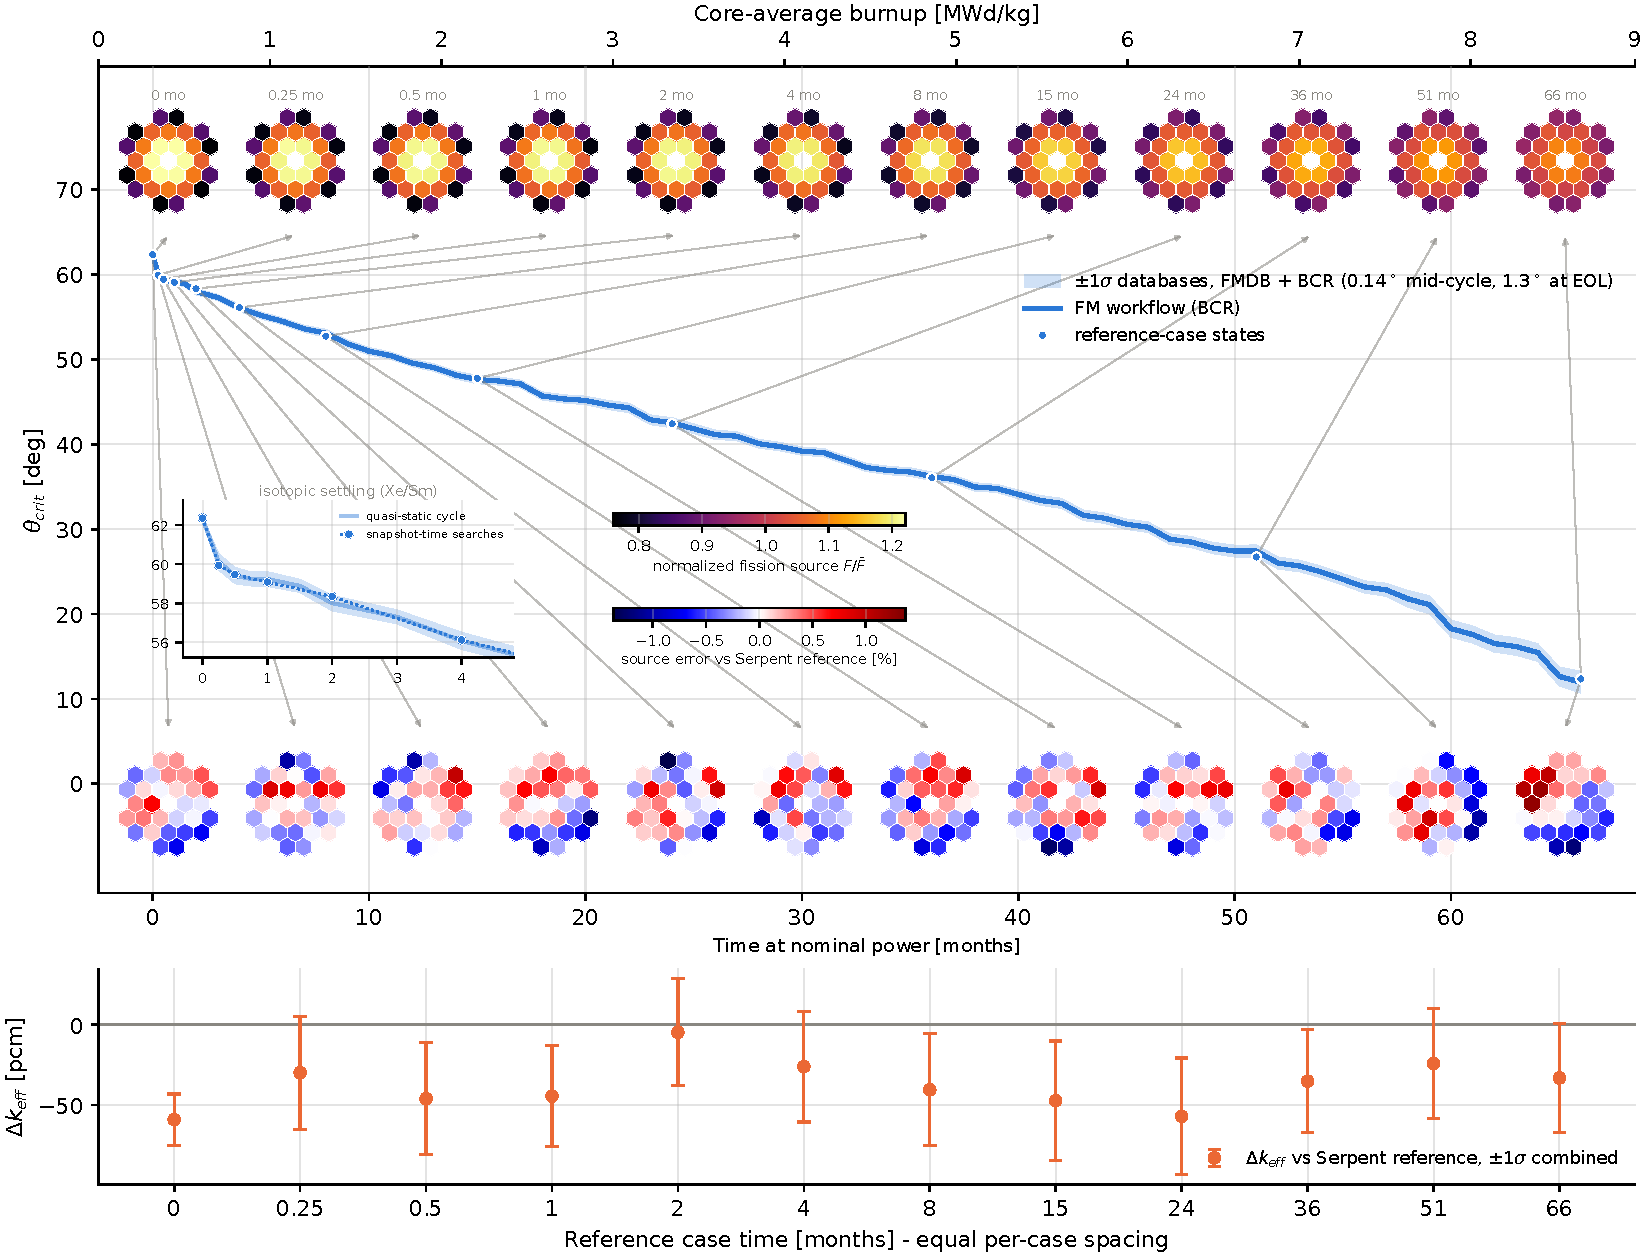
\includegraphics[width=\textwidth]{figures/critical_drum_angle_over_the_cycle_with_maps.pdf}
    \caption{Critical drum angle over the cycle at \SI{2}{MW} (core-average burnup on the upper axis), with the $\pm1\sigma$ band from the fifty database realizations and the twelve states at which the reference calculations were run. For each of those states: the normalized fission source of the workflow (upper maps) and its assembly-wise error against the Serpent 2 reference (lower maps). The inset resolves the first months, where the isotopic settling takes place, and compares the quasi-static cycle with searches run directly at the snapshot times. Bottom panel: deviation of the workflow $k_{\rm eff}$ from the reference at the twelve states, with the combined $\pm1\sigma$ uncertainty; the cases are equally spaced for readability.}
    \label{fig:cycle}
\end{figure}

\subsection{Excess reactivity and cycle length}

The reactivity with the drums fully extracted, evaluated along the cycle, sets the cycle length at its crossing of unity (\Cref{fig:drumsout}). It starts at 2870 pcm at BOL, a value read from the tallied database and not a free parameter. It decreases by 500 pcm per year over the second year and by 376 pcm per year at the end of the window (307 and 231 pcm per MWd/kg), and 120 pcm are left at 66 months: end of life falls near month 70. The reference points are the snapshot transports themselves, full-statistics calculations at $\theta = \ang{0}$ with the composition of each snapshot. They are tallied at the reference temperature state, while the workflow curve carries the evolved profile; the difference is bounded in Section~\ref{sec:hyp}. The maps in \Cref{fig:drumsout} show the flattening of the fission source over the cycle: the assembly peaking factor decreases from 1.221 to 1.097, the centre loses \SI{11}{\percent} and the drum-adjacent periphery gains \SI{21}{\percent}. The assembly-wise error of the workflow source against the reference is \SI{0.24}{\percent} on average. The depletion output gives the inventory behind this. At 66 months $^{235}$U is depleted by \SI{5.75}{\percent} core-wide (\SI{6.6}{\percent} in the most exposed assembly), $^{239}$Pu builds up to \SI{1.05}{\percent} of the initial $^{235}$U, and its share of the fissions reaches \SI{3.6}{\percent}.

\begin{figure}[ht!]
    \centering
    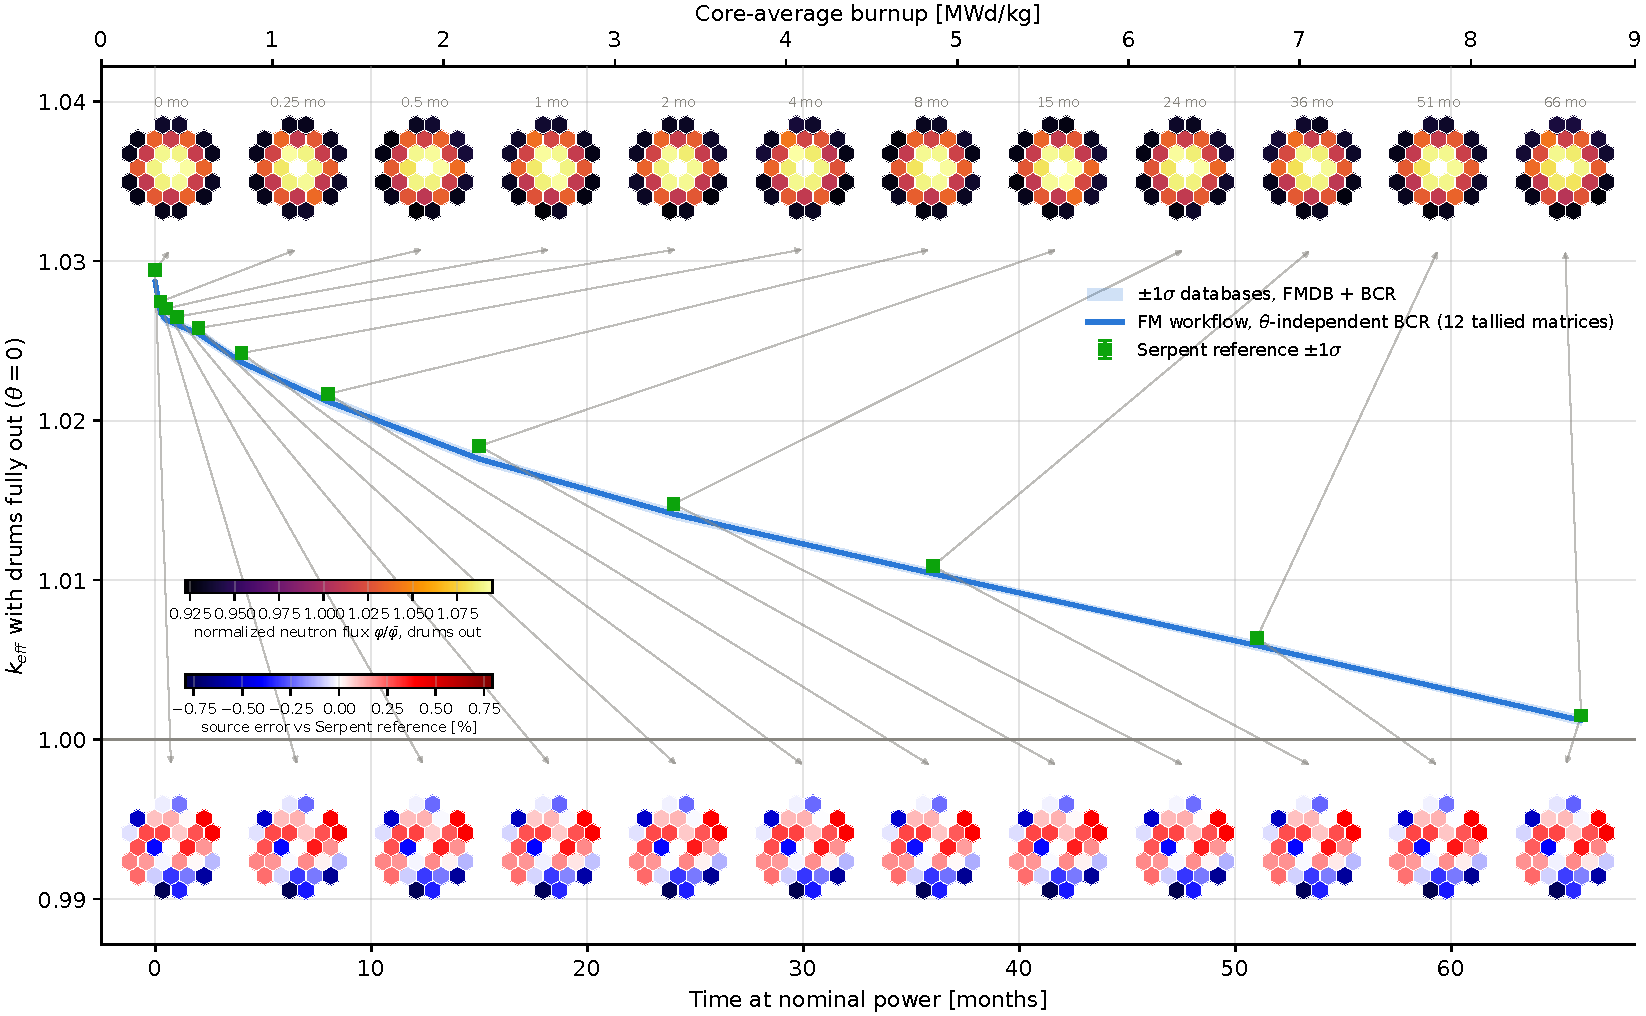
\includegraphics[width=\textwidth]{figures/excess_reactivity_with_the_drums_fully_extracted.pdf}
    \caption{$k_{\rm eff}$ with the drums fully extracted over the cycle: FM workflow with its $\pm1\sigma$ band and the twelve reference Serpent 2 calculations. For each reference time, and with the drums fully extracted, the normalized fission source of the workflow (top row) and its assembly-wise error against the reference (bottom row); the drums are out here, whereas the maps of \Cref{fig:cycle} are at the critical drum position of each time.}
    \label{fig:drumsout}
\end{figure}

\subsection{The three assumptions of the factorization, measured}\label{sec:hyp}

\paragraph{Angle independence.} The production snapshots are tallied at a single drum angle. To measure what this costs, the snapshot compositions of the same restart file were re-tallied at four more angles, \ang{45}, \ang{90}, \ang{135} and \ang{180}: 48 transports and no additional depletion. The test compares tallied matrices only, with no interpolation. At each angle $\theta'$ and snapshot time $t_s$,
\begin{equation}
    \Delta k(\theta', t_s) \;=\; k\big[\,a^{\rm tally}(\theta',0)\cdot BCR(t_s)\,\big] \;-\; k\big[\,a^{\rm tally}(\theta', t_s)\,\big],
    \label{eq:thetatest}
\end{equation}
the hypothesis on the left, the truth on the right. Each point carries the statistics of four independent tallies, about 22 pcm on $k_{\rm eff}$. The 44 measured points (\Cref{fig:theta}) have an RMS of 23 pcm and none is beyond 59 pcm; the angle means are $-19$, $+11$, $+5$ and $+2$ pcm, with no trend in burnup or angle. The hypothesis holds at the resolution of the test at every angle, the \ang{180} corner included, which is where a shutdown-margin evaluation would apply the BCR farthest from its tally point. The effect on the deliverable was also checked, by running the cycle with the BCR interpolated between the five tallied angles. The critical angle differs from the single-angle cycle by \ang{0.69} on average and \ang{1.54} at most, at 24 months; through the local drum worth of 55 pcm per degree, that maximum is 85 pcm, dominated by the tally noise of the additional planes.

\begin{figure}[ht!]
    \centering
    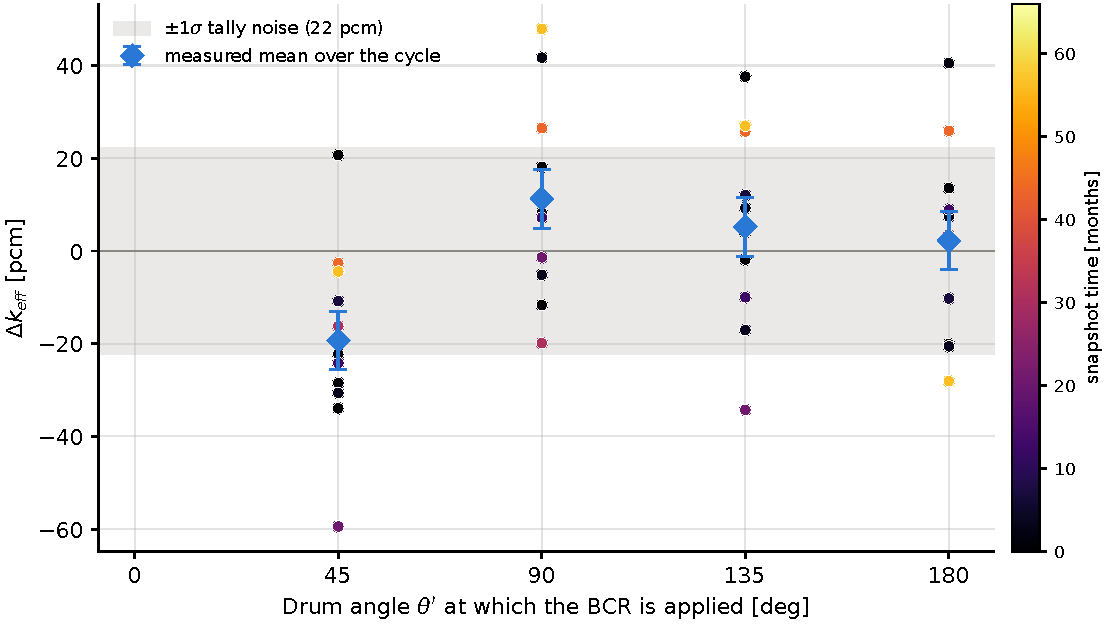
\includegraphics[width=0.75\textwidth]{figures/independence_hypothesis_structural_error_measured.pdf}
    \caption{Structural error of the angle-independent BCR, Eq.~\eqref{eq:thetatest}, at the four drum angles where the snapshot compositions were re-tallied: one point per snapshot time (colour), the mean over the cycle with its standard error, and the $\pm1\sigma$ band expected from the statistics of the four tallies in each point.}
    \label{fig:theta}
\end{figure}

\paragraph{Frozen temperature.} The snapshots are tallied at the frozen nominal temperature state, so the BCR isolates the composition effect. The temperature dependence is carried by the $(T,\theta)$ interpolation; letting the snapshots follow the evolving profile would count it twice. What the factorization neglects is the cross-term between temperature and burnup. It was measured with one dedicated transport: the 51-month composition re-tallied with the workflow-evolved temperature profile (a redistribution of up to \SI{+10}{K} as the source flattens), against the reference-state snapshot with the same composition, the same drum angle and an independent seed. The result is $\Delta k_{\rm eff} = -9 \pm 15$ pcm, statistically zero. The dominant BCR coefficients have the same median in the two cases, 0.9775 against 0.9776, and their differences are distributed as the tally noise predicts.

\paragraph{Single history.} The production depletion runs with the drums fully extracted, while the operating reactor keeps them on the critical trajectory. With the drums inserted, the flux in the drum-adjacent periphery is depressed and those assemblies accumulate exposure more slowly. The hypothesis was measured with a second depletion, identical to the first except for the drums, frozen at \ang{33.75}, the database angle closest to the time average of the critical trajectory. Its compositions were re-tallied at the standard conditions at five snapshot times. Table~\ref{tab:history} gives the effect on the tallied matrices and the effect that survives in the workflow, where the BCR from the alternative history replaces the production one on the interpolated matrix. The compositions move $k_{\rm eff}$ by at most 27 pcm, with a sign change around mid-cycle. The workflow moves by at most 58 pcm at mid-cycle and by 3 pcm at end of life: the cycle length, read at the drums-out crossing, is insensitive to the drum history assumed in the depletion. The two depletions also act as a replicate of the composition chain: the core-total $^{235}$U inventory reproduces to \SI{0.013}{\percent} between independent seeds, so the low-statistics depletion is not a source of error.

\begin{table}[ht!]
    \centering
    \caption{Single-history test: $k_{\rm eff}$ with the drums-inserted depletion history minus $k_{\rm eff}$ with the production history, on the tallied matrices and in the workflow (pcm). Each entry carries the statistics of two and four independent tallies respectively, about 16 and 22 pcm.}
    \label{tab:history}
    \begin{tabular}{lcccc}
        \toprule
        \textbf{Time (months)} & \textbf{8} & \textbf{24} & \textbf{51} & \textbf{66} \\
        \midrule
        Tallied matrices & $+22$ & $+27$ & $-26$ & $-26$ \\
        Workflow         & $+54$ & $+58$ & $+4$  & $+3$  \\
        \bottomrule
    \end{tabular}
\end{table}

\subsection{Density of the snapshot grid}

How many snapshot times are needed is answered with the acceptance method used for the FMDB selection in Ref.~\cite{vita2026fm}. Nested sub-grids of the twelve-point grid are tested at the midpoints of the full grid, where the time-interpolation error peaks. At each test time the workflow gives the critical state on the full database, and every sub-grid is evaluated at that frozen state, so $\Delta k_{\rm eff}$ isolates the effect of the density. The full grid reproduces the states it defined to 0.4 pcm, the search tolerance. The interpolation error falls from 297 pcm with 2 snapshot times to 80 pcm with 4 and to 21 pcm with 7, where it first enters the 22 pcm band of the reference statistics (\Cref{fig:grid}). Seven snapshot times are therefore sufficient on the burnup axis of this design. Beyond that, the residual is dominated by the tally noise the BCR carries as a ratio of two independent runs; more snapshot times would not reduce it.

\begin{figure}[ht!]
    \centering
    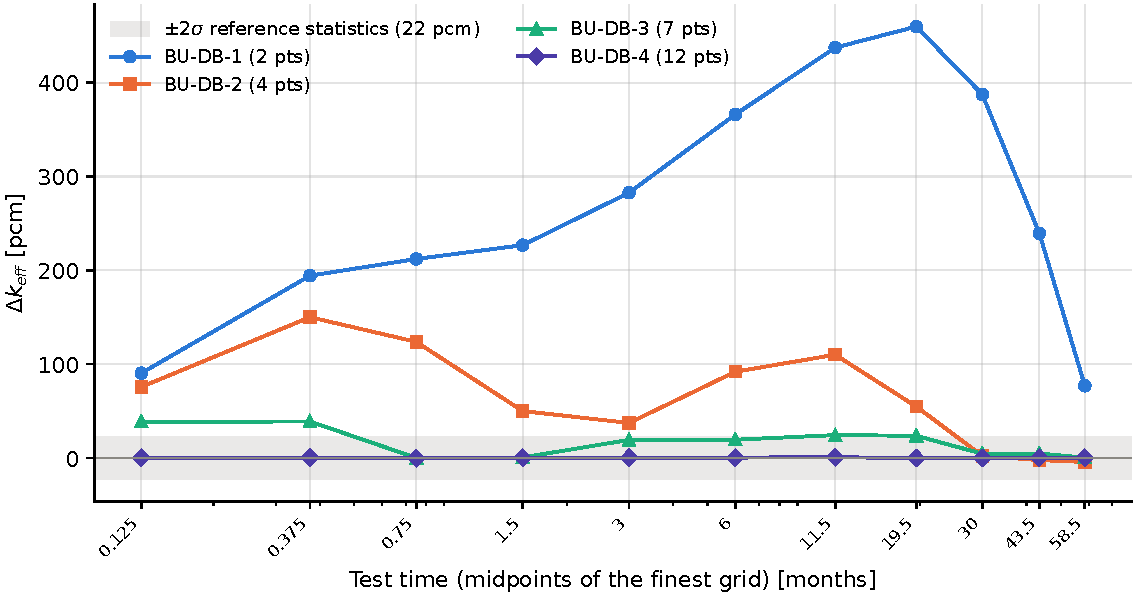
\includegraphics[width=0.7\textwidth]{figures/interpolation_error_vs_snapshot_grid_density.pdf}
    \caption{Time-interpolation error of nested snapshot grids of 2, 4, 7 and 12 points, evaluated at the midpoints of the full grid at the critical state given by the workflow, compared with the statistics of the reference calculations.}
    \label{fig:grid}
\end{figure}

\section{Conclusions}\label{sec:concl}

The fission matrix criticality search of Ref.~\cite{vita2026fm} has been extended to fuel burnup without adding an axis to its database. Burnup enters the interpolated matrix as a multiplicative correction ratio, tallied once per snapshot time at a single reference angle and temperature state. One low-statistics depletion gives the compositions, and twelve independent full-statistics transports, restarted from it, tally the snapshot matrices at 66 CPU\,h each. The workflow then drives a quasi-static cycle in which drum position, temperature profile, fission source and cell-wise burnup are updated together at every step: 18 seconds on one core for a 66-month cycle, uncertainty ensemble included.

Reference criticality calculations at the states returned by the algorithm put $k_{\rm eff}$ within $-59$ to $-5$ pcm of unity over the cycle. The bias is already present at beginning of life and shows no trend with burnup; the assembly-wise fission source agrees to about one percent. The three assumptions of the factorization were measured on dedicated campaigns, all restarted from the same depletion. The angle independence of the BCR holds at the 22 pcm resolution of the test at every drum angle up to \ang{180}. The temperature--burnup cross-term is $-9 \pm 15$ pcm. The drum history behind the compositions moves the workflow by at most 58 pcm at mid-cycle and by 3 pcm at end of life. Seven snapshot times suffice on the burnup axis. Statistical uncertainties are propagated to every result with an ensemble of fifty database realizations; the drum-angle bands widen from \ang{0.14} to \ang{1.3} as the drums approach full extraction.

The residual of the method is the $(T,\theta)$ interpolation of the original database, not the burnup correction. The power-to-temperature correlation is shared by the workflow and the references, so the present verification cannot see it; replacing it with a thermal response from a conduction solver is the natural next step, and the interface of the workflow already allows it. The construction does not depend on the power level: the temperature axis of the database carries the power dependence, and the same snapshot database serves the search at any power.

\section*{ACKNOWLEDGEMENTS}
%%% TODO: funding and acknowledgements

\bibliographystyle{ANStopical}
\bibliography{main}

\end{document}
